\documentclass[12pt,oneside]{article} % Uma Coluna e lingua portuguesa
%\usepackage[T1]{fontenc}        % Permite digitar os acentos de forma normal
\usepackage[utf8]{inputenc}
%\usepackage[english]{babel}
\usepackage[portuges,brazil]{babel}
%\usepackage[latin1]{inputenc}
\usepackage[dvips]{graphicx}    % Permite Gráficos
%\usepackage{times}    % Fonte Times
\usepackage{fancyhdr}
\usepackage{array}
\usepackage{multicol}
\usepackage[colorlinks=true,linkcolor=blue,urlcolor=blue]{hyperref}
\usepackage{nomencl}    % glossario
\usepackage{amssymb}
\usepackage{amsmath}
\usepackage[compact]{titlesec}
\usepackage{wrapfig}
\usepackage{color}

%=======================================================================

% Hifenização das palavras desconhecidas pelo LaTeX
%\hyphenation{}
\paperheight    297mm
\paperwidth     210mm
\voffset         -15mm
\headheight      15pt %% tamanho de letra
\headsep         5mm  %% para o início do texto
\oddsidemargin  -3.0mm
\evensidemargin -3.0mm
\textwidth      167.0mm
\topmargin      005.0mm
\textheight     240.0mm
\footskip       10.0mm

\title{SAET 2023 - Maratona de Programação}

\author{Maratona de Programação}
\date{26 de Outubro de 2022}
\usepackage{indentfirst}
\usepackage{subfig}

\parindent=0pt
\setlength{\parskip}{7pt plus 1pt minus 2pt}
\titlespacing{\section}{0pt}{*0}{*0}
\titlespacing{\subsection}{0pt}{*0}{*0}
\titlespacing{\subsubsection}{0pt}{*0}{*0}

\begin{document}

\begin{center}
\textbf{\Huge SAET 2023 - Maratona de Programação} \\
\vspace{0.2cm}
\textit{26 de Outubro de 2022} \\
\vspace{1.0cm}
%\textbf{Sevidor BOCA:} \\
%\texttt{\large http://maratona.c3sl.ufpr.br/boca/} \\
%\vspace{1.0cm}
\begin{figure}[h!]
	\centering
 
\includegraphics[scale=0.95]{capa.png}
\end{figure}
\vspace{1.0cm}
%\textbf{Organizadores:}\\
%{\small Flávio Zavan} \\
%{\small Ricardo Oliveira} \\
\vspace{1.0cm}
\end{center}

\clearpage

\pagestyle{fancy}
\renewcommand{\footrulewidth}{0.7pt}
\renewcommand{\headrulewidth}{0.7pt}
\lhead{SAET 2023 - Maratona de Programação}
%\chead{Maratonas de Programação}
\rhead{26 de Outubro de 2023}
\cfoot{\thepage}

\newpage

% Espaco para o create-zips.sh nao achar
  \section*{Instruções Importantes}

\begin{itemize}

    \item Use a opção \textbf{Runs} para enviar suas soluções. Os problemas podem resolvidos em qualquer ordem e
    linguagem (dentre C, C++ e Python, independentemente do problema);

    \item Suas soluções serão testadas com várias entradas,
    além das dada como exemplo. Por isso, sua solução pode não ser
    aceita mesmo se funcionar para os exemplos dados. Certifique-se que ela
    funciona para todas as entradas possíveis;

    \item A saída gerada deve ser \textit{exatamente} conforme
    especificada. Em particular, \textbf{não} imprima instruções (``digite um
            número'', ``a resposta é'', etc);

    \item É garantido que todas as entradas usadas para teste estarão de acordo
    com o enunciado, não sendo necessário testar se são válidas;

    \item Ao enviar uma solução, o sistema irá responder uma das
    seguintes respostas:
    \begin{itemize}
        \item \verb|Not answered yet|: a solução está sendo corrigida.
        Aguarde um pouco e atualize a página;
        \item \verb|YES|: solução aceita. Parabéns!
        \item \verb|Wrong Answer|: a saída impressa pelo seu programa não é a
        saída correta esperada, para alguma entrada de teste;
        \item \verb|Presentation Error|: a saída impressa está correta, exceto
        por espaços em branco e/ou quebras-de-linha faltando/sobrando;
        \item \verb|Time Limit Exceeded|: o tempo de execução do seu programa
        ultrapassou o tempo limite estipulado para o problema (ver tabela
        abaixo). O tempo de execução da sua solução precisa ser menor;
        \item \verb|Runtime Error|: seu programa gerou algum erro em tempo de
        execução (``crashou'');
        \item \verb|Compile Error|: seu programa não compila.
    \end{itemize}

    \item Todas as linhas, tanto na entrada quanto na saída, terminam com o
    caractere de fim-de-linha ($\backslash n$), mesmo quando houver apenas uma única
    linha na entrada e/ou saída;

    \item Sua solução deve processar cada arquivo de entrada no tempo máximo
    estipulado para cada problema, dado pela seguinte tabela:

    \begin{table}[h]
    \centering
    \begin{tabular}{|c|c||c|}
    \hline
    \textbf{Problema} & \textbf{Nome} & \textbf{Tempo Limite (segundos)} \\
    \hline
    A & Alergia & 1 \\
    \hline
    B & Jogo & 1 \\
    \hline
    C & Vasilha Errada & 1 \\
    \hline
    D & Drawkcabackward & 1 \\
    \hline
    E & Empilha Copos & 1 \\
    \hline
    F & Falco & 1 \\
    \hline
    G & Gafe & 1 \\
    \hline
    K & Tiras & 1 \\
    \hline
    L & Lista & 1 \\
    \hline
    M & Meuzamigo & 1 \\
    \hline
    \end{tabular}
    \end{table}

\end{itemize}

\newpage
\section*{A: Alergia } %tle=1
\vspace{-0.52cm}
\noindent \begin{verbatim}Arquivo: jogo.[c|cpp|py]\end{verbatim}
Alergia não é coisa só de humano não, a bicharada também sofre.

Maya tem um cachorrinho parceiro e super animal chamado Thomy. Ele tem o costume de cantar de galo, mandando Maya lhe dar comida. Claro que tudo em "cachorrês", afinal, ele é um cachorro! Animal é quem não entende ele.

Sempre forte como um touro, hoje Thomy amanheceu andando como uma barata tonta pela casa... deu zebra! Maya não poderia deixá-lo desamparado, pois não tem sangue de cobra e é uma mãe coruja com os seus bichinhos. Não titubeou: como uma lebre o levou para a veterinária.

O doutor prescreveu uma nova ração, já que Thomy havia desenvolvido alergia a alguns ingredientes. Ofereceram uma ração lá do Peru, que era o olho da cara... mais caro que um boi! Nem que a vaca tussa que Maya iria pagar tudo aquilo.

Ela procurou outra veterinária, e lá eles prescreveram uma ração bem mais barata, uma pechincha. Tão barata que ela desconfiou, e pediu para você confirmar se algum dos ingredientes da ração poderia causar uma reação no cachorrinho. Mostre quem é o bicho da programação, criando um programa que compare os ingredientes presentes na ração e as alergias do Thomy!

\subsection*{Entrada}
A primeira linha tem apenas um inteiro $N$ ($1\leq N \leq 100$), o número de ingredientes.

A segunda linha contém $N$ inteiros $R_i$ ($1\leq i \leq N$). Se $R_i=1$, então a ração contém o ingrediente $i$. Se $R_i=0$, então ela não contém o ingrediente $i$.

A terceira linha contém $N$ inteiros $A_i$, indicando se Thomy tem alergia ao ingrediente $i$. Se $A_i=1$, então Thomy tem alergia ao ingrediente $i$. Se $A_i=0$, então ele não tem alergia ao ingrediente $i$.

\subsection*{Saída}
Imprima \texttt{"S"} (maiúsculo e sem aspas) se Maya pode dar a ração para o Thomy.

Imprima \texttt{"N"} (maiúsculo e sem aspas) se Maya não deve dar a ração para o Thomy.

%----- Exemplo 1 -----%
\newpage
\begin{table}[!h]
\centering
\begin{tabular}{|l|l|}
\hline
\begin{minipage}[t]{3in}
\textbf{Exemplo de entrada}
\begin{verbatim}
6
1 0 0 1 1 0 
0 0 1 0 0 1 
\end{verbatim}
\vspace{1mm}
\end{minipage}
&
\begin{minipage}[t]{3in}
\textbf{Exemplo de saída}
\begin{verbatim}
S
\end{verbatim}
\vspace{1mm}
\end{minipage} \\
\hline
\end{tabular}
\end{table}

%----- Exemplo 2 -----%
\begin{table}[!h]
\centering
\begin{tabular}{|l|l|}
\hline
\begin{minipage}[t]{3in}
\textbf{Exemplo de entrada}
\begin{verbatim}
4
1 1 1 1
0 1 0 0
\end{verbatim}
\vspace{1mm}
\end{minipage}
&
\begin{minipage}[t]{3in}
\textbf{Exemplo de saída}
\begin{verbatim}
N
\end{verbatim}
\vspace{1mm}
\end{minipage} \\
\hline
\end{tabular}
\end{table}


\newpage
\section*{B: Jogo } %tle=1
\vspace{-0.52cm}
\noindent \begin{verbatim}Arquivo: jogo.[c|cpp|py]\end{verbatim}
    Carlos e Pedro gostam muito de futebol e querem jogar uma partida um contra o outro. Como ambos são goleiros, eles precisam de jogadores no ataque e na defesa para completar o seu time.

    Para isso, eles têm uma lista de jogadores interessados em participar da partida, contendo os
pontos de ataque e de defesa de todos. Quem tem seus pontos de defesa maior que os de ataque, joga na defesa,
caso contrário, joga no ataque.

    Para a divisão ser justa, a escolha dos jogadores será feitas em rodadas. Carlos e Pedro escolherão um jogador por rodada.
Na primeira rodada Carlos escolhe um jogador primeiro, na segunda Pedro escolhe primeiro e vão intercalando até acabarem os jogadores. Caso o número de jogadores
seja ímpar, um não será escolhido.

    A cada rodada a escolha é feita de forma bem simples:
\begin{itemize}
    \item Quem tiver a maior quantidade de pontos somados é escolhido;
    \item Se alguém do ataque e da defesa tem a mesma quantidade de pontos, ambos têm preferência pelo atacante;
    \item Caso tenha mais jogadores do ataque escolhidos, se possível, um jogador da defesa será escolhido;
    \item Caso tenha mais jogadores da defesa escolhidos, se possível, um jogador do ataque será escolhido;
\end{itemize}

\subsection*{Entrada}

A primeira linha da entrada contém o número de jogadores a serem escolhidos $N$ ($2\leq N\leq 10^5$).
Cada uma das $N$ linhas seguintes contêm 2 inteiros: $K_i$ e $M_i$ ($0\leq K_i\leq 99, 0\leq M_i\leq 99$), sendo, respectivamente. os pontos de ataque
e de defesa do jogador $i$.  

\subsection*{Saída}

A saída deverá conter uma linha com a média do time com a maior quantidade de pontos somados, com truncamento em duas casas decimais.

%----- Exemplo 1 -----%
\newpage
\begin{table}[!h]
\centering
\begin{tabular}{|l|l|}
\hline
\begin{minipage}[t]{3in}
\textbf{Exemplo de entrada}
\begin{verbatim}
4
10 20
30 10
10 50
10 5
\end{verbatim}
\vspace{1mm}
\end{minipage}
&
\begin{minipage}[t]{3in}
\textbf{Exemplo de saída}
\begin{verbatim}
37.50
\end{verbatim}
\vspace{1mm}
\end{minipage} \\
\hline
\end{tabular}
\end{table}

%----- Exemplo 2 -----%
\begin{table}[!h]
\centering
\begin{tabular}{|l|l|}
\hline
\begin{minipage}[t]{3in}
\textbf{Exemplo de entrada}
\begin{verbatim}
6
62 1
79 65
71 71
 8 91
71 99
20 24
\end{verbatim}
\vspace{1mm}
\end{minipage}
&
\begin{minipage}[t]{3in}
\textbf{Exemplo de saída}
\begin{verbatim}
125.00
\end{verbatim}
\vspace{1mm}
\end{minipage} \\
\hline
\end{tabular}
\end{table}

%----- Exemplo 3 -----%
\begin{table}[!h]
\centering
\begin{tabular}{|l|l|}
\hline
\begin{minipage}[t]{3in}
\textbf{Exemplo de entrada}
\begin{verbatim}
10
61 55
49 81
96 23
 2 59
56 41
33 20
93 16
72 20
65 66
58 94
\end{verbatim}
\vspace{1mm}
\end{minipage}
&
\begin{minipage}[t]{3in}
\textbf{Exemplo de saída}
\begin{verbatim}
117.40
\end{verbatim}
\vspace{1mm}
\end{minipage} \\
\hline
\end{tabular}
\end{table}


\newpage
\section*{C: Vasilha Errada } %tle=1
\vspace{-0.52cm}
\noindent \begin{verbatim}Arquivo: vasilhaerrada.[c|cpp|py]\end{verbatim}
Nathan é um menino apaixonado por triângulos, por conta disso em sua casa só tem vasilhas triangulares. Contudo, sua mãe Ana sempre faz panquecas circulares para o seu filho levar para escola. Como Nathan é ruim em matemática ele nunca sabe qual o melhor recipiente para levar. Por sorte no seu material escolar há uma régua, conseguindo dessa forma medir os lados de todas as vasilhas da casa. Sendo assim, o seu trabalho 
será criar um programa que lê as medidas de Nathan e mostrá-lo quais são os raios limites que a panqueca pode ter para cada recipiente. 

\begin{figure}[h!]
	\centering
 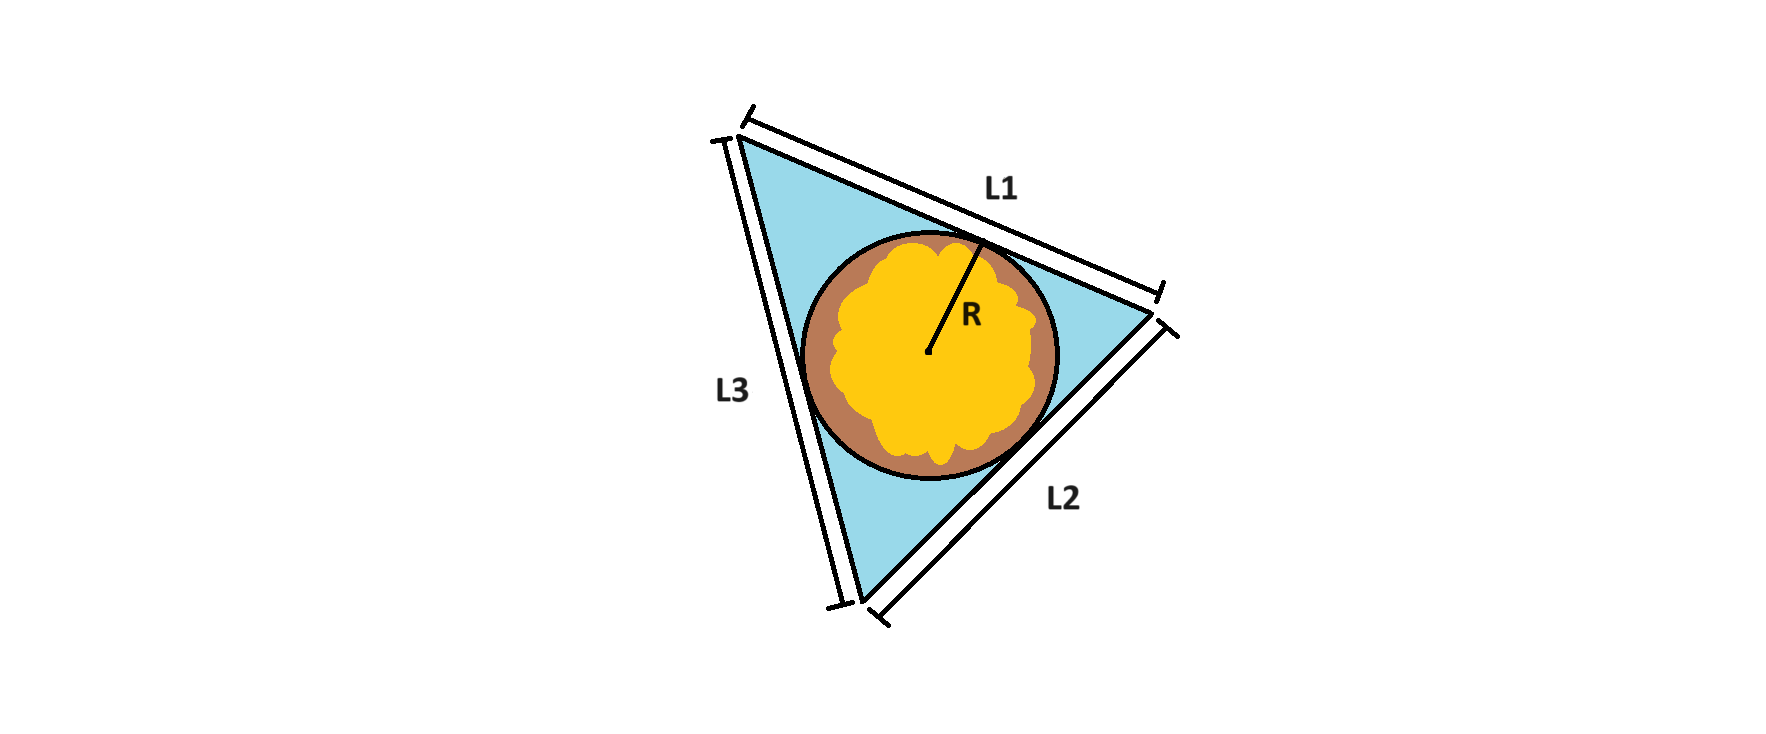
\includegraphics[scale=0.5]{vasilhaerrada.png}
\end{figure}

\subsection*{Entrada}
 
A primeira linha da entrada contém o número $N$ ($1\leq N\leq 1000$) de vasilhas.
 
As próximas $N$ linhas conterá os valores de $L1, L2, L3$ ($1\leq L1, L2, L3 \leq 500$) em cm representando as medidas realizadas por Nathan em cada recipiente. Considere que Nathan não erre as medidas e que a precisão pode alcançar duas casas decimais.
 
\subsection*{Saída}
A saída deverá conter $N$ números, sendo um valor por linha, que serão os raios R máximos, com duas casas decimais, que a panqueca pode ter em cada vasilha apresentado por Nathan.

%----- Exemplo 1 -----%
%\newpage
\begin{table}[!h]
\centering
\begin{tabular}{|l|l|}
\hline
\begin{minipage}[t]{3in}
\textbf{Exemplo de entrada}
\begin{verbatim}
6
3 4 5
12 12 12
10 12 10
2.08 1.82 1.30
33.07 96.2 103.86
131.27 316.33 216.7
\end{verbatim}
\vspace{1mm}
\end{minipage}
&
\begin{minipage}[t]{3in}
\textbf{Exemplo de saída}
\begin{verbatim}
1.00
3.46
3.00
0.45
13.61
33.24
\end{verbatim}
\vspace{1mm}
\end{minipage} \\
\hline
\end{tabular}
\end{table}


\newpage
\section*{D: Drawkcabackward} %tle=1
\vspace{-0.52cm}
\noindent \begin{verbatim}Arquivo: drawkcab.[c|cpp|py]\end{verbatim}
Uma das mais divertidas tarefas de um maratonista de programação é a escolha do
nome da sua equipe. Depois de muito debate, sua equipe decidiu escolher o nome
da seguinte maneira:

\begin{itemize}
    \item O nome deverá ser uma substring não vazia de uma dada string $s$;
    \item O nome deverá ser palíndrome (isto é, deve ser igual quando lido da
            esquerda para a direita e da direita para a esquerda);
    \item Cada letra do alfabeto $a$, $b$, $c$, ..., $z$ tem um \textit{valor}
    $V_a$, $V_b$, $V_c$, ..., $V_z$. O \textit{valor total} do nome escolhido é a soma dos valores de
    suas letras. O nome escolhido deverá ter o maior valor total possível.
\end{itemize}

Como exemplo, considere a string $s = $ \verb|xabaydcbbcdyz| e os valores
$V_a = 20$, $V_b = -10$, $V_c = 15$, $V_d = 11$, $V_x = 20$, $V_y = -20$ e $V_z
= 20$. Alguns nomes que poderiam ser escolhidos são:

\begin{itemize}
    \item \verb|aba|, com valor total $V_a + V_b + V_a = 20-10+20 = 30$;
    \item \verb|dcbbcd|, com valor total $11 + 15 - 10 - 10 + 15 + 11 = 32$;
    \item \verb|ydcbbcdy|, com valor total $-20 + 11 + 15 - 10 - 10 + 15 + 11
    -20 = -8$;
    \item Outras substrings palíndromes de $s$.
\end{itemize}

Neste exemplo, a substring palíndrome \verb|dcbbcd| tem o maior valor total
possível (32), e portanto este será o nome da equipe.

Dada a string $s$ e os valores de cada letra, ajude a escolher o nome da sua
equipe!

\subsection*{Entrada}

A primeira linha contém 26 valores inteiros $V_a, V_b, V_c, ..., V_z$ (entre
        $-1000$ e $1000$ cada) indicando o
valor de cada letra do alfabeto.

A segunda linha contém a string $s$ ($1 \leq |s| \leq 5 \times 10^5$), contendo
apenas letras minúsculas.

\subsection*{Saída}

Imprima uma única linha contendo o valor total do nome escolhido pela equipe.

\newpage
\begin{table}[!h]
\centering
\hspace{-2cm}
\begin{tabular}{|l|l|}
\hline
\begin{minipage}[t]{5.5in}
\textbf{Exemplo de entrada}
\begin{verbatim}
20 -10 15 11 0 0 0 0 0 0 0 0 0 0 0 0 0 0 0 0 0 0 20 0 -20 20
xabaydcbbcdyz
\end{verbatim}
\vspace{1mm}
\end{minipage}
&
\begin{minipage}[t]{1.5in}
\textbf{Exemplo de saída}
\begin{verbatim}
32
\end{verbatim}
\vspace{1mm}
\end{minipage} \\
\hline
\end{tabular}
\end{table}

\begin{table}[!h]
\centering
\hspace{-2cm}
\begin{tabular}{|l|l|}
\hline
\begin{minipage}[t]{5.5in}
\textbf{Exemplo de entrada}
\begin{verbatim}
1 -1 0 0 0 0 0 0 0 0 0 0 0 0 0 0 0 0 0 0 0 0 0 0 0 0
bbbaaaaaabbbbbbaaa
\end{verbatim}
\vspace{1mm}
\end{minipage}
&
\begin{minipage}[t]{1.5in}
\textbf{Exemplo de saída}
\begin{verbatim}
6
\end{verbatim}
\vspace{1mm}
\end{minipage} \\
\hline
\end{tabular}
\end{table}

\begin{table}[!h]
\centering
\hspace{-2cm}
\begin{tabular}{|l|l|}
\hline
\begin{minipage}[t]{5.5in}
\textbf{Exemplo de entrada}
\begin{verbatim}
7 1 1 8 1 -5 1 1 3 1 -10 1 71 -42 1 1 1 1 1 1 1 1 1 1 1 1
lazafakeekafdrawkcabackwardlaza
\end{verbatim}
\vspace{1mm}
\end{minipage}
&
\begin{minipage}[t]{1.5in}
\textbf{Exemplo de saída}
\begin{verbatim}
31
\end{verbatim}
\vspace{1mm}
\end{minipage} \\
\hline
\end{tabular}
\end{table}

\begin{table}[!h]
\centering
\hspace{-2cm}
\begin{tabular}{|l|l|}
\hline
\begin{minipage}[t]{5.5in}
\textbf{Exemplo de entrada}
\begin{verbatim}
-1 0 0 0 0 0 0 0 0 0 0 0 0 0 0 0 0 0 0 0 0 0 0 0 0 0
aaaaaaaaaaaaaaaaaaaaaaaaaaaaaaaaaaaaaaaaaaaaaaaaaaaa
\end{verbatim}
\vspace{1mm}
\end{minipage}
&
\begin{minipage}[t]{1.5in}
\textbf{Exemplo de saída}
\begin{verbatim}
-1
\end{verbatim}
\vspace{1mm}
\end{minipage} \\
\hline
\end{tabular}
\end{table}


\newpage
\section*{E: Empilha Copos} %tle=1
\vspace{-0.52cm}
\noindent \begin{verbatim}Arquivo: empilha.[c|cpp|py]\end{verbatim}
Um professor de matemática que é fascinado por competições resolveu fazer uma
dinâmica com a sua turma. Ele percebeu que em sua casa havia uma grande
quantidade de copos, e optou por utilizá-los em sua próxima aula.

Ele explicou da
seguinte maneira para os seus alunos: Dado $N$ copos ($1 \leq N \leq 10000$), eles
devem determinar qual o maior valor de $B$ tal que é possível formar um
triângulo de base $B$ utilizando no máximo $N$ copos.

Como exemplo, a figura abaixo mostra que, com no máximo $N=8$ copos, é possível formar um
triângulo de base $B=3$:

\begin{center}
    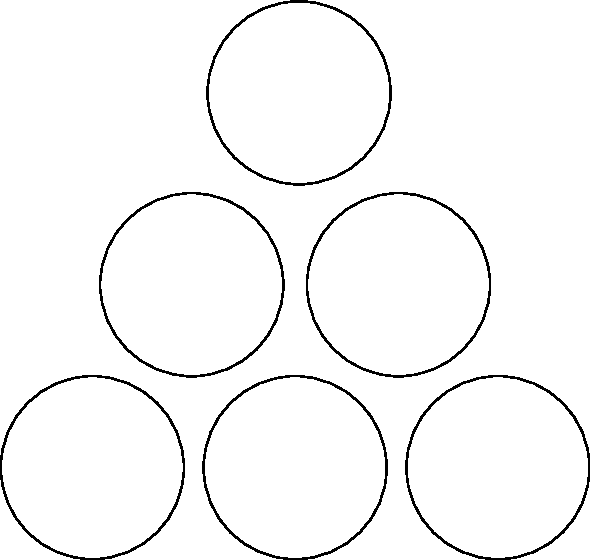
\includegraphics[scale=0.2]{empilha/empilha.pdf}
\end{center}

Neste exemplo, 6 copos são usados e 2 são descartados.

\subsection*{Entrada}

A entrada contém apenas um inteiro $N$ ($1 \leq N \leq 10000$).

\subsection*{Saída}

Imprima o maior valor de $B$ tal que é possível formar um triângulo de base $B$
usando até $N$ copos.

%----- Exemplo 1 -----%
\begin{table}[!h]
\centering
\begin{tabular}{|l|l|}
\hline
\begin{minipage}[t]{3in}
\textbf{Exemplo de entrada}
\begin{verbatim}
10
\end{verbatim}
\vspace{1mm}
\end{minipage}
&
\begin{minipage}[t]{3in}
\textbf{Exemplo de saída}
\begin{verbatim}
4
\end{verbatim}
\vspace{1mm}
\end{minipage} \\
\hline
\end{tabular}
\end{table}

%----- Exemplo 2 -----%
\begin{table}[!h]
\centering
\begin{tabular}{|l|l|}
\hline
\begin{minipage}[t]{3in}
\textbf{Exemplo de entrada}
\begin{verbatim}
8
\end{verbatim}
\vspace{1mm}
\end{minipage}
&
\begin{minipage}[t]{3in}
\textbf{Exemplo de saída}
\begin{verbatim}
3
\end{verbatim}
\vspace{1mm}
\end{minipage} \\
\hline
\end{tabular}
\end{table}

%----- Exemplo 3 -----%
\begin{table}[!h]
\centering
\begin{tabular}{|l|l|}
\hline
\begin{minipage}[t]{3in}
\textbf{Exemplo de entrada}
\begin{verbatim}
1000
\end{verbatim}
\vspace{1mm}
\end{minipage}
&
\begin{minipage}[t]{3in}
\textbf{Exemplo de saída}
\begin{verbatim}
44
\end{verbatim}
\vspace{1mm}
\end{minipage} \\
\hline
\end{tabular}
\end{table}


\newpage
\section*{F: Falco} %tle=1
\vspace{-0.52cm}
\noindent \begin{verbatim}Arquivo: falco.[c|cpp|py]\end{verbatim}
Agente Falco é um experiente espião da Nlogonia, especializado em infiltrações. Para se comunicar com seus aliados ele utiliza mensagens codificadas na cifra de César, uma técnica de criptografia simples, mas eficaz.

A cifra de César é uma técnica de criptografia que envolve a substituição de cada letra do alfabeto por outra letra, deslocada um número fixo de posições. Por exemplo, com um deslocamento de 3 posições, a letra "A" se torna "D", a letra "B" se torna "E" e assim por diante. O deslocamento é um segredo compartilhado com o destinatário da mensagem.

Sua tarefa é desenvolver um programa que codifica uma mensagem de texto usando a cifra de César com um deslocamento especificado para o Agente Falco.
\subsection*{Entrada}
 
A primeira linha da entrada  contém 2 inteiros $t$ ($0 < t \leq 100$) e $k$ ($0 < t \leq 10^6$), sendo respectivamente o tamanho da mensagem e o deslocamento.
 
A segunda linha contém a mensagem $s$, composta apenas de caracteres minúsculos.
 
\subsection*{Saída}
A saida deverá ser a mensagem codificada.

%----- Exemplo 1 -----%
\begin{table}[!h]
\centering
\begin{tabular}{|l|l|}
\hline
\begin{minipage}[t]{3in}
\textbf{Exemplo de entrada}
\begin{verbatim}
9
4 1
aaaa
\end{verbatim}
\vspace{1mm}
\end{minipage}
&
\begin{minipage}[t]{3in}
\textbf{Exemplo de saída}
\begin{verbatim}
bbbb
\end{verbatim}
\vspace{1mm}
\end{minipage} \\
\hline
\end{tabular}
\end{table}

%----- Exemplo 2 -----%
\begin{table}[!h]
\centering
\begin{tabular}{|l|l|}
\hline
\begin{minipage}[t]{3in}
\textbf{Exemplo de entrada}
\begin{verbatim}
4 3
saet
\end{verbatim}
\vspace{1mm}
\end{minipage}
&
\begin{minipage}[t]{3in}
\textbf{Exemplo de saída}
\begin{verbatim}
vdhw
\end{verbatim}
\vspace{1mm}
\end{minipage} \\
\hline
\end{tabular}
\end{table}

%----- Exemplo 3 -----%
\begin{table}[!h]
\centering
\begin{tabular}{|l|l|}
\hline
\begin{minipage}[t]{3in}
\textbf{Exemplo de entrada}
\begin{verbatim}
1 27
a
\end{verbatim}
\vspace{1mm}
\end{minipage}
&
\begin{minipage}[t]{3in}
\textbf{Exemplo de saída}
\begin{verbatim}
b
\end{verbatim}
\vspace{1mm}
\end{minipage} \\
\hline
\end{tabular}
\end{table}


\newpage
\section*{G: Gafe} %tle=1
\vspace{-0.52cm}
\noindent \begin{verbatim}Arquivo: gafe.[c|cpp|py]\end{verbatim}
Gabriel fez aniversário semana retrasada, e tudo o que ele queria de presente era um fone de ouvido. Não tinha dúvidas sobre o que desejar no momento de apagar as velas do seu bolinho de aniversário. 

A festa ia começar, quando a SAET (Serviço de Aplicação e Execução Tática), um dos departamentos da polícia federal, invadiu equivocadamente a sua casa, pensando que se tratava do domicílio de um dos criminosos mais procurados do país. Tudo ocorreu por causa do cabo Paradella, que confundiu o número 66 por 50 nas evidências. Este erro desencadeou uma série de eventos que culminaram em uma incursão à casa de Gabriel. Que gafe!

Após perceberem o erro, a comandante do esquadrão deu de presente um dos fones de ouvidos táticos usados pela polícia como pedido de desculpas ao Gabriel. Apesar de super tecnológico, não tem um botão de desligar. Ao invés disso, tem três botões capazes de diminuir o nível do volume de formas muito inconvencionais:

\begin{itemize}
\item \textbf{Botão \texttt{E-}}: Diminui o nível do lado esquerdo em 1. Não faz nada se o nível já for 0;
\item \textbf{Botão \texttt{D-}}: Diminui o nível do lado direito em 1. Não faz nada se o nível já for 0;
\item \textbf{Botão S}: Subtrai o nível do lado mais alto pelo nível do lado mais baixo. Se os volumes forem iguais, um lado qualquer é subtraído do outro.
\end{itemize}

Para exemplificar, se o volume do fone estiver nos níveis [880, 980], o botão \texttt{E-} o fará mudar para os níveis [879, 980], o botão \texttt{D-} para [880, 979], e o botão \texttt{S} para [880, 100].

Acontece que o nível de cada lado é \textit{independente} e vai até $1000$, e Gabriel não quer ficar apertando os botões milhares de vezes até desligar o fone. Dado os níveis do fone no momento, crie um programa que ajude Gabriel, dizendo a quantidade mínima de vezes que ele terá de apertar os botões para desligar completamente o seu novo fone de ouvido.

\subsection*{Entrada}
A entrada contém apenas uma linha com dois inteiros $E$ e $D$ ($0 \leq E, D \leq 1000$), o volume do lado esquerdo e direito do fone, respectivamente.

\subsection*{Saída}
Imprima uma única linha contendo a quantidade mínima de vezes que Gabriel terá de apertar os botões para desligar ambos lados do fone.

%----- Exemplo 1 -----%
\newpage
\begin{table}[!h]
\centering
\begin{tabular}{|l|l|}
\hline
\begin{minipage}[t]{3in}
\textbf{Exemplo de entrada}
\begin{verbatim}
2 2
\end{verbatim}
\vspace{1mm}
\end{minipage}
&
\begin{minipage}[t]{3in}
\textbf{Exemplo de saída}
\begin{verbatim}
3
\end{verbatim}
\vspace{1mm}
\end{minipage} \\
\hline
\end{tabular}
\end{table}

%----- Exemplo 2 -----%
\begin{table}[!h]
\centering
\begin{tabular}{|l|l|}
\hline
\begin{minipage}[t]{3in}
\textbf{Exemplo de entrada}
\begin{verbatim}
11 15
\end{verbatim}
\vspace{1mm}
\end{minipage}
&
\begin{minipage}[t]{3in}
\textbf{Exemplo de saída}
\begin{verbatim}
8
\end{verbatim}
\vspace{1mm}
\end{minipage} \\
\hline
\end{tabular}
\end{table}

%----- Exemplo 3 -----%
\begin{table}[!h]
\centering
\begin{tabular}{|l|l|}
\hline
\begin{minipage}[t]{3in}
\textbf{Exemplo de entrada}
\begin{verbatim}
1000 976
\end{verbatim}
\vspace{1mm}
\end{minipage}
&
\begin{minipage}[t]{3in}
\textbf{Exemplo de saída}
\begin{verbatim}
48
\end{verbatim}
\vspace{1mm}
\end{minipage} \\
\hline
\end{tabular}
\end{table}


\newpage
\section*{K: Tiras } %tle=1
\vspace{-0.52cm}
\noindent \begin{verbatim}Arquivo: tiras.[c|cpp|py]\end{verbatim}
Sila trabalha em um pequeno ateliê de costura próprio onde é confeccionado de tudo, desde camisetas e uniformes até o vestuário infantil. Depois de uma semana cheia de entregas, a maior cooperativa da cidade, SAET (Sociedade de Agropecuária e Empreendedorismo de Tumingapurubá), pediu para que ela produzisse bodies para bebês, pois o departamento de Recursos Humanos da cooperativa queria dar um de presente para toda funcionária ou cooperada gestante que entrasse de licença maternidade. 

Para confeccionar os bodies, existem $n$ caixas com tiras de comprimento $c_i$. Sila pediu para que seu marido, Amário, cortasse essas tiras em tamanhos iguais, sem deixar sobras e procurando deixar as tiras o mais compridas possível. Para fazer isso, Amário criou o seguinte processo para juntar duas caixas adjacentes:

\begin{itemize}
    \item Pegar duas caixas adjacentes $i$ e $i+1$ com tiras de comprimentos $c_i$ e $c_{i+1}$;
    \item Cortar todas as tiras das duas caixas para que os pedaços fiquem com tamanho MDC$(c_i, c_{i+1})$, onde MDC é a operação Máximo Divisor Comum;
    \item Substituir as duas caixas $i$ e $i+1$ por uma caixa com as tiras de tamanho MDC$(c_i, c_{i+1})$ recém cortadas.
\end{itemize}

Para ter uma noção de quanto Amário irá demorar, Sila mandou que você determinasse qual é o mínimo de vezes que o processo de junção terá de ser realizado para que, ao final, todas as tiras das caixas remanescentes tenham o mesmo tamanho. Note que a quantidade de tiras não importa, mas sim o tamanho delas em cada caixa.

Por exemplo, se houverem $n=5$ caixas, cada uma com tiras de comprimento $c=[10,30,12,42,2]$, o processo pode ser realizado um mínimo de 3 vezes até que, ao final, todas as caixas tenham tiras de mesmo comprimento e o processo não possa mais ser realizado. Uma das formas de juntar as caixas 3 vezes, satisfazendo o pedido de Sila, é:

\begin{center}
    $[\textcolor{red}{10},\textcolor{red}{30},12,42,2] \rightarrow [10,\textcolor{red}{12},\textcolor{red}{42},2] \rightarrow [\textcolor{red}{10},\textcolor{red}{6},2] \rightarrow [2,2]$
\end{center}

Em vermelho, estão o comprimento das tiras das duas caixas escolhidas para realizar a junção.

\subsection*{Entrada}
 
A primeira linha da entrada contém o número de caixas $n$ ($2\leq n\leq 10^5$).
 
A próxima linha consiste em $n$ inteiros $c_i$ ($1\leq c_i \leq 10^5$), o tamanho das tiras dentro da caixa $i$.
 
\subsection*{Saída}
A saída deverá conter uma linha com o número de processos de junção realizados, atendendo à ordem de Sila.

%----- Exemplo 1 -----%
\newpage
\begin{table}[!h]
\centering
\begin{tabular}{|l|l|}
\hline
\begin{minipage}[t]{3in}
\textbf{Exemplo de entrada}
\begin{verbatim}
5
10 30 12 42 2
\end{verbatim}
\vspace{1mm}
\end{minipage}
&
\begin{minipage}[t]{3in}
\textbf{Exemplo de saída}
\begin{verbatim}
3
\end{verbatim}
\vspace{1mm}
\end{minipage} \\
\hline
\end{tabular}
\end{table}

%----- Exemplo 2 -----%
\begin{table}[!h]
\centering
\begin{tabular}{|l|l|}
\hline
\begin{minipage}[t]{3in}
\textbf{Exemplo de entrada}
\begin{verbatim}
5
16 4 4 2 8
\end{verbatim}
\vspace{1mm}
\end{minipage}
&
\begin{minipage}[t]{3in}
\textbf{Exemplo de saída}
\begin{verbatim}
4
\end{verbatim}
\vspace{1mm}
\end{minipage} \\
\hline
\end{tabular}
\end{table}

%----- Exemplo 3 -----%
\begin{table}[!h]
\centering
\begin{tabular}{|l|l|}
\hline
\begin{minipage}[t]{3in}
\textbf{Exemplo de entrada}
\begin{verbatim}
3
1 1 100000
\end{verbatim}
\vspace{1mm}
\end{minipage}
&
\begin{minipage}[t]{3in}
\textbf{Exemplo de saída}
\begin{verbatim}
1
\end{verbatim}
\vspace{1mm}
\end{minipage} \\
\hline
\end{tabular}
\end{table}


\newpage
\section*{L: Lista } %tle=1
\vspace{-0.52cm}
\noindent \begin{verbatim}Arquivo: lista.[c|cpp|py]\end{verbatim}
Pedro tem uma clínica que funciona 7 dias por semana, porém ele não gosta
de trabalhar muito aos finais de semana, e por isso pediu para sua secretária
distribuir os seus $N$ pacientes de acordo com a primeira letra de seus nomes em
certos dias da semana.

Ele atende as pessoas que têm os nomes que começam
com as letras A,B,C e D no domingo; já na segunda-feira ele atende as pessoas que têm
os nomes que começar com as letras E,F,G,e H; e assim por diante até
a sexta-feira, quando só atende as pessoas com as letras U, V e W , e no sábado X,
Y e Z .

Entretanto, ele pediu para sua secretária que não organizasse os pacientes,
    dentro de um mesmo dia, em ordem
alfabética, pois assim seria injusto com os pacientes que marcaram suas consultas
antes. Dentro de um mesmo dia, a lista de pacientes deve seguir a ordem em que
marcaram as consultas.

Assim, por exemplo, se Caio, Felipe, Diego,
Ana, Bianca, Alice e Tiago marcaram consultas (nessa ordem),
seriam atendidos no domingo, nessa ordem: Caio, Diego, Ana, Bianca e Alice;
Já Felipe seria atendido na segunda-feira, portanto após todos esses; Tiago
seria atendido por último.

\subsection*{Entrada}

A primeira linha contém $N$ ($1 \leq N \leq 1000$), o número de pacientes. As
próximas $N$ linhas contém um nome cada, na ordem em que marcaram as consultas.
Os nomes serão strings de até 20 letras minsculas e/ou maiusculas cada.

\subsection*{Saída}

Imprima um nome de paciente por linha, na ordem em que serão atendidos.

%----- Exemplo 1 -----%
\begin{table}[!h]
\centering
\begin{tabular}{|l|l|}
\hline
\begin{minipage}[t]{3in}
\textbf{Exemplo de entrada}
\begin{verbatim}
5
bruna
Gabi
ana
Caio
bianca
\end{verbatim}
\vspace{1mm}
\end{minipage}
&
\begin{minipage}[t]{3in}
\textbf{Exemplo de saída}
\begin{verbatim}
bruna
ana
Caio
bianca
Gabi
\end{verbatim}
\vspace{1mm}
\end{minipage} \\
\hline
\end{tabular}
\end{table}


\newpage
\section*{M: Meuzamigo } %tle=1
\vspace{-0.52cm}
\noindent \begin{verbatim}Arquivo: meuzamigo.[c|cpp|py]\end{verbatim}
A universidade Blupen está oferecendo uma gincana com várias brincadeiras 
de premiações interessantes. Uma delas é a Meuzamigo e nosso amigo 
Manoel Gomes está decidido a ganhar. A brincadeira consiste em
em $N$ pessoas conectadas a $N-1$ fios. O participante é o primeiro a se conectar a rede,
em seguida os ajudantes da gincana se conectam para dar vida a brincadeira. 

Para vencer, é necessário que o participante 
diga qual é a distância mais longa entre ele mesmo e um ajudante qualquer. 
É garantido que todos as pessoas estejam conectadas na rede.

\subsection*{Entrada}
 
A primeira linha da entrada contém o número de pessoas $N$ ($2\leq n\leq 10^5$).
 
As próximas $N-1$ linhas contém $A$ e $B$, as conexões entre cada particante.
 
\subsection*{Saída}
A saída deverá conter um número inteiro correspondente a distância mais longa
entre Manoel Gomes e algum participante.

%----- Exemplo 1 -----%
\begin{table}[!h]
\centering
\begin{tabular}{|l|l|}
\hline
\begin{minipage}[t]{3in}
\textbf{Exemplo de entrada}
\begin{verbatim}
9
1 9
1 4
9 5
4 3
5 6
1 2
1 7
5 8
\end{verbatim}
\vspace{1mm}
\end{minipage}
&
\begin{minipage}[t]{3in}
\textbf{Exemplo de saída}
\begin{verbatim}
3
\end{verbatim}
\vspace{1mm}
\end{minipage} \\
\hline
\end{tabular}
\end{table}

%----- Exemplo 2 -----%
\begin{table}[!h]
\centering
\begin{tabular}{|l|l|}
\hline
\begin{minipage}[t]{3in}
\textbf{Exemplo de entrada}
\begin{verbatim}
2
1 2
\end{verbatim}
\vspace{1mm}
\end{minipage}
&
\begin{minipage}[t]{3in}
\textbf{Exemplo de saída}
\begin{verbatim}
1
\end{verbatim}
\vspace{1mm}
\end{minipage} \\
\hline
\end{tabular}
\end{table}

%----- Exemplo 3 -----%
\begin{table}[!h]
\centering
\begin{tabular}{|l|l|}
\hline
\begin{minipage}[t]{3in}
\textbf{Exemplo de entrada}
\begin{verbatim}
19
1 7
7 12
12 6
1 14
6 13
13 17
14 9
12 2
14 18
1 10
10 8
13 11
1 15
13 16
1 4
6 5
7 19
2 3
\end{verbatim}
\vspace{1mm}
\end{minipage}
&
\begin{minipage}[t]{3in}
\textbf{Exemplo de saída}
\begin{verbatim}
5
\end{verbatim}
\vspace{1mm}
\end{minipage} \\
\hline
\end{tabular}
\end{table}


\end{document}
